% --------------------------------------------------------------------------------

\begin{exercise}[\hl{Implementation Task: Racetrack (Exercise 5.12)}]

Consider driving a race car around a turn like those shown in Figure 5.5.
You want to go as fast as possible, but not so fast as to run off the track.
In our simplified racetrack, the car is at one of a discrete set of grid
positions, the cells in the diagram. The velocity is also discrete, a
number of grid cells moved horizontally and vertically per time step.
The actions are increments to the velocity components. Each may be changed
by $+1,-1$ or $0$ in each step, for a total of nine ($3 \times 3$) actions.
Both velocity components are restricted to be nonnegative and less than $5$,
and they cannot both be zero except at the starting line. Each episode
begins in one of the randomly selected start states with both velocity
components zero and ends when the car crosses the finish line. The rewards
are $-1$ for each step until the car crosses the finish line. If the car
hits the track boundary, it is moved back to a random position on the starting line,
both velocity components are reduced to zero, and the episode continues.
Before updating the car's location at each time step, check to see if the
projected path of the car intersects the track boundary. It it intersects
the finish line, the episode ends; if it intersects anywhere else, the car
is considered to have hit the track boundary and is sent back to the starting line.
To make the task more challenging, with probability $0.1$ at each time step
the velocity increments are both zero, independently of the indented increments.
Apply a Monte Carlo control method to this task to compute the optimal policy from
each starting state. Exhibit several trajectories following the optimal
policy (but turn the noise off for these trajectories).

\begin{figure}[H]
  \centering
  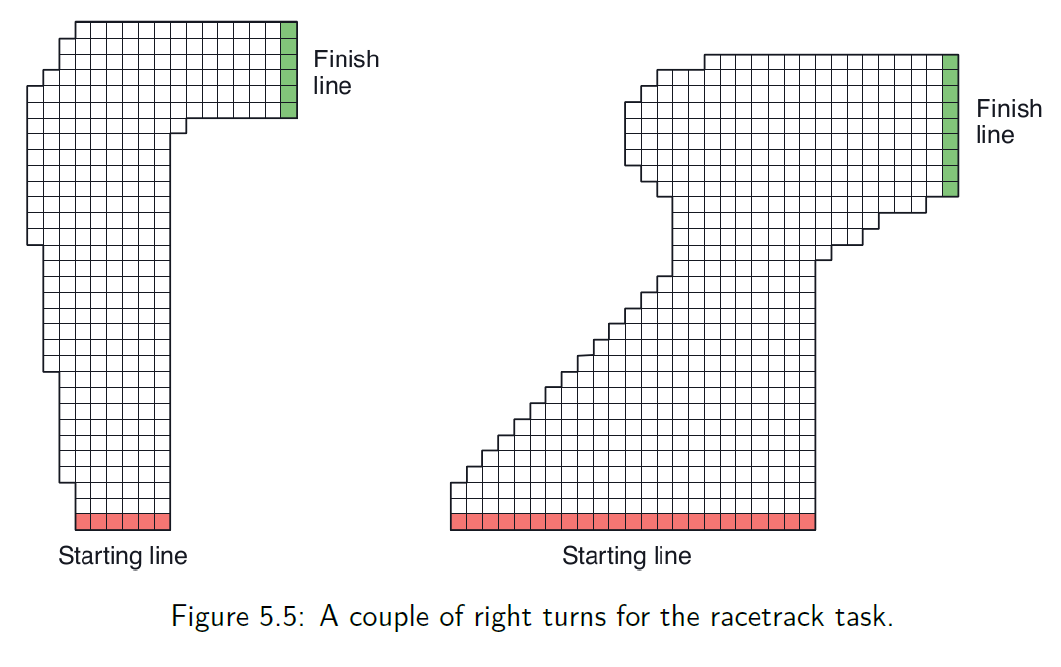
\includegraphics[width = 0.6 \textwidth]{figure_5.5.png}
\end{figure}

\end{exercise}

% --------------------------------------------------------------------------------

\begin{solution}

\phantom{}

\end{solution}

% --------------------------------------------------------------------------------
